% Auth: Nicklas Vraa
% Docs: https://github.com/NicklasVraa/LiX

\documentclass{textbook}

\lang      {english}
\title     {Modeling, Simulation and Optimization}
\subtitle  {(For the Layman)}
\author    {Jaime Torres}
\cover*    {resources/textbook_front.pdf}{resources/textbook_back.pdf}
\license   {CC}{by-nc-sa}{3.0}{The Company}
\isbn      {978-0201529838}
\publisher {Nobodym just me!}
\edition   {1}{2024}
\dedicate  {Myself}{Because I'm cool}
\thank     {Thank you to me for being the best}
\keywords  {optimization, simulation, python, mathematical modeling}

\begin{document}

\tableofcontents

\chapter{Mathematical Modeling.}

For this chapter, we'll:

\begin{itemize}
    \item Get our framework from an algorithmic framework of thinking to algebraic 
    framework
    \item Represent a problem with algebraic expressions.
    \item Make proper implementations of mathematical models.
\end{itemize}

\section{Introduction to mathematical modeling}

Before we can begin to think about models, we must understand what they are.
And, for the purposes of this book, we can define a mathematical model as a representation
of a real life problem with an abstract representation of the phenomenons we intend to study.

For an immediately relevant example, a lot of problems in graph theory can be explained in algebraic terms.
Although these problems can be a bit more mathematical in nature, then we can use them to explain real-life problems.
Such as:

\begin{itemize}
    \item Shortest path in a graph, for computer networking and pathfinding.
    \item The traveling salesman problem, for pathfinding, DNA sequencing and microchip manufacturing 
    \item The vehicular routing problem, for finding multiple instances of a TSP-esque solution on a same graph
\end{itemize}

As a practical example of such a graph-based problem, let's analyze the following:

\subsection{Example 1: The transport problem}

Let a finite number of sources and a finite number of destinations, we can determine the
number of elements we can route to every destination with a minimal cost for every source. 
For example, if we said such sources are factories and the destinations are warehouses, we could see a 3x3
graph as it follows:

% \includegraphics[options]{name}

\subsection{Example 2: Cover problems}

More than a specific problem, this is a subdivisio of problems meant to cover a certain group of demands
or coverage criteria according to a specific defined problem.

\subsubsection{The hospital problem}

For example, say we got a group of neighborhoods that are of euclidian behavior, and we intend to put the minimum amount of
hospitals that can cover the entire region we're considering. A hospital covers the neighborhood is located on and
those who share a boundary with it. A boundary is a non-zero

For an example, imagine the following instance of this problem:

%% answer is 5 and 8

\subsubsection{The four color theorem}

The four color theorem is a very famous application of a cover problem. 

% 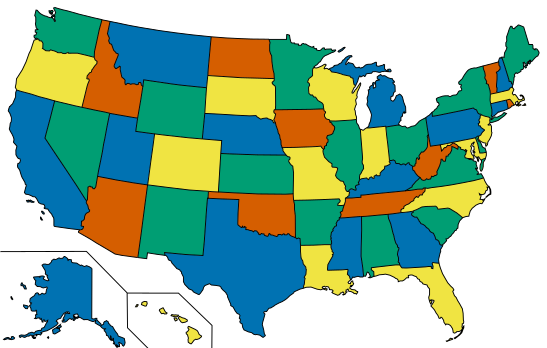
\includegraphics[scale=0.4]{notes/resources/Map_of_United_States_accessible_colors_shown}

\subsection{Example 3: Minimum spanning tree}

If we imagine a tree data structure such as a graph with no cycles, and a graph as an interlocked set of
nodes, a minimum spanning tree would be the minimum cost path that can connect all nodes as a tree.

This problem has a set of requirements for it to be considered correct:

\begin{itemize}
    \item There must be no cycles or subcycles in the solution
    \item the number of connections must be the number of nodes minus one
\end{itemize}

\section{Classification of mathematical models}

These models can be, as most things in mathematics, categorized and calificated in 

\subsection{Deterministic mathematical models}

These are models that can be predicted in a way that is certain.

\subsection{Stochastic mathematicam models}

A stochastic model is one that involves a certain amount of randomness. For example, 

\subsection{Static mathematical models}

A static model is one that does not depend on time, implying that whatever time passes, the result of
such a system should stay constant. Generally this will happen for models where we don't even consider time as a 
relevant variable.

\subsection{Dynamic mathematical models}
\subsubsection{Continuous time models}

A continuous time model is one where we assume time as a continuous function, that meaning, it is
flowing in somewhat real time. Although the way computation has it should bring it to be a finite level of
statuses, this should be a big enough sample such as we can assume the variable can be statistically generalized into
a continuous system

\subsubsection{Discrete time models}

A fairly interesting application of discrete time models comes from finance, where there exists 
capitalization in a set time interval. For example, we could imagine the free cash flow of an economic project as
a mathematical problem to be optimized, such as this:

\subsubsection{Continuous status models}

In a continuous status model, the dependant variable can assume any value in the range of a specific interval.

\subsubsection{Discrete status models}

In these models, the difference is analogous to the way a discrete time model varies from a continuous
time model. Values for the dependant variable shouls only assume specific values in an interval. For example, a
model where every value the dependant variable can take is in the range of natural numbers ($\mathbb{N}$) would be 
a discrete status.

\subsubsection{Examples of model classification}

\paragraph{Number of attendants in a bank every hour}

This example would be a dynamic mathematical model where every 

\paragraph{Temperature of a classroom every hour}

For this, 

\subsection{Open mathematical models}

An open mathematical model is one where the input that is recieved will be external to this model and
independent from itself. For example a translator, such as Google Translate or DeepL will model natural language
such as the input recieved is not eventually retroactively giving feedback to the model. Although it is possible that
in ML models there are eventually expected use cases introduced into the model, for out purposes, they will be considered 
open as long as at runtime the previous example does not feedback into further answers.




%\includegraphics[options]{name}

\section{}

\end{document}
